% !TEX TS-program = pdflatex
%\documentclass[draftcls, onecolumn, journal]{IEEEtran}
\documentclass[journal]{IEEEtran}
%\documentclass[a4paper,11pt]{article}
%\usepackage{fullpage}

%\renewcommand{\baselinestretch}{1.9}
\usepackage[hidelinks]{hyperref}
\usepackage{graphicx}
\usepackage{color}
\usepackage{amsmath}
\usepackage{subcaption}
\usepackage{algorithmicx}
\usepackage{algorithm}
\usepackage{algpseudocodex}
\usepackage{cleveref}
\usepackage{diagbox}
%\usepackage{multicol}
%\usepackage{cite}
\usepackage[
style=ieee,
sorting=ynt
]{biblatex}
\graphicspath{images/}
\addbibresource{sources.bib}


\newcommand{\argmax}[1]{\underset{#1}{\operatorname{arg}\,\operatorname{max}}\;}

%\bibliographystyle{IEEEtran}

%%%%%%%%%%%%%%%%%%%%%%%%%%%%%%%%%%%%%%%%%%%%%%%%%%%%%%%%%%%%%%%%%%%%%%
\title{Fan-Beam Computerized Tomography Simulation}

\author{Kutay Ugurlu}

%%%%%%%%%%%%%%%%%%%%%%%%%%%%%%%%%%%%%%%%%%%%%%%%%%%%%%%%%%%%%%%%%%%%%%
\begin{document}
%\renewcommand{\baselinestretch}{1.6}

\maketitle

\begin{abstract}This project report demonstrates the implementation of Fan Beam Computerized Tomography simulation. The effect of different design parameters including the length of the detector, the number of beams and the angle between consecutive projections is inspected and discussed comparatively in both quantitative and qualitative manner. The work is derived from the previously developed code in Parallel Beam X-Ray Computerized Tomography \cite{ugurlu2021}. The developed software and GUI to run it can be found in \href{https://github.com/kutay-ugurlu/Fan-Beam-Computerized-Tomography-Simulation}{github.com/kutay-ugurlu/Fan-Beam-Computerized-Tomography-Simulation} \\
%\textit{Keywords:} Inverse electrocardiography, electrocacardiographic imaging, statistical estimation, Bayesian estimation, Kalman filter.
\end{abstract}
\begin{IEEEkeywords}
	imaging, medical imaging, X-Ray computerized tomography, image reconstruction
\end{IEEEkeywords}

\section{Introduction} \label{sec:intro}
The purpose of this project report is to demonstrate the procedure followed to simulate Fan-Beam Projected X-Ray Computerized Tomography. This project report consists of \nameref{sec:theory}, \nameref{sec:implementation}, \nameref{sec:results} and \nameref{sec:discuss} sections. The second section introduces the technical background for the CT simulation and the following section illustrates the algorithm using pseudocode snippets. \nameref{sec:results} and \nameref{sec:discuss} section presents the comparative results regarding different user-specified parameters with the conclusion and reasons behind them.

\subsection{History}
The history of X-Ray Computerized Tomography can be dated back to 1917, when an Austrian mathematician called Johann Radon invented an algorithm, referred to as Radon transform today, on how to calculate line integrals in a two-dimensional section. The idea of computed tomography was developed in 1967 and was first used in a medical setting was in 1971 \cite{richmond2004sir}, by Godfrey Hounsfield. The device was tested at
James Ambrose’s department at Atkinson Morley Hospital in Wimbledon. This first model did not include a computer, instead the waves was written on a magnetic tape of the device EMI Scanner CT1010 in Figure \ref{fig:CT1010}. It was in 1973 that commercial CT scanners were available to the public. \cite{CTHist}

\begin{figure}[h]
\centering
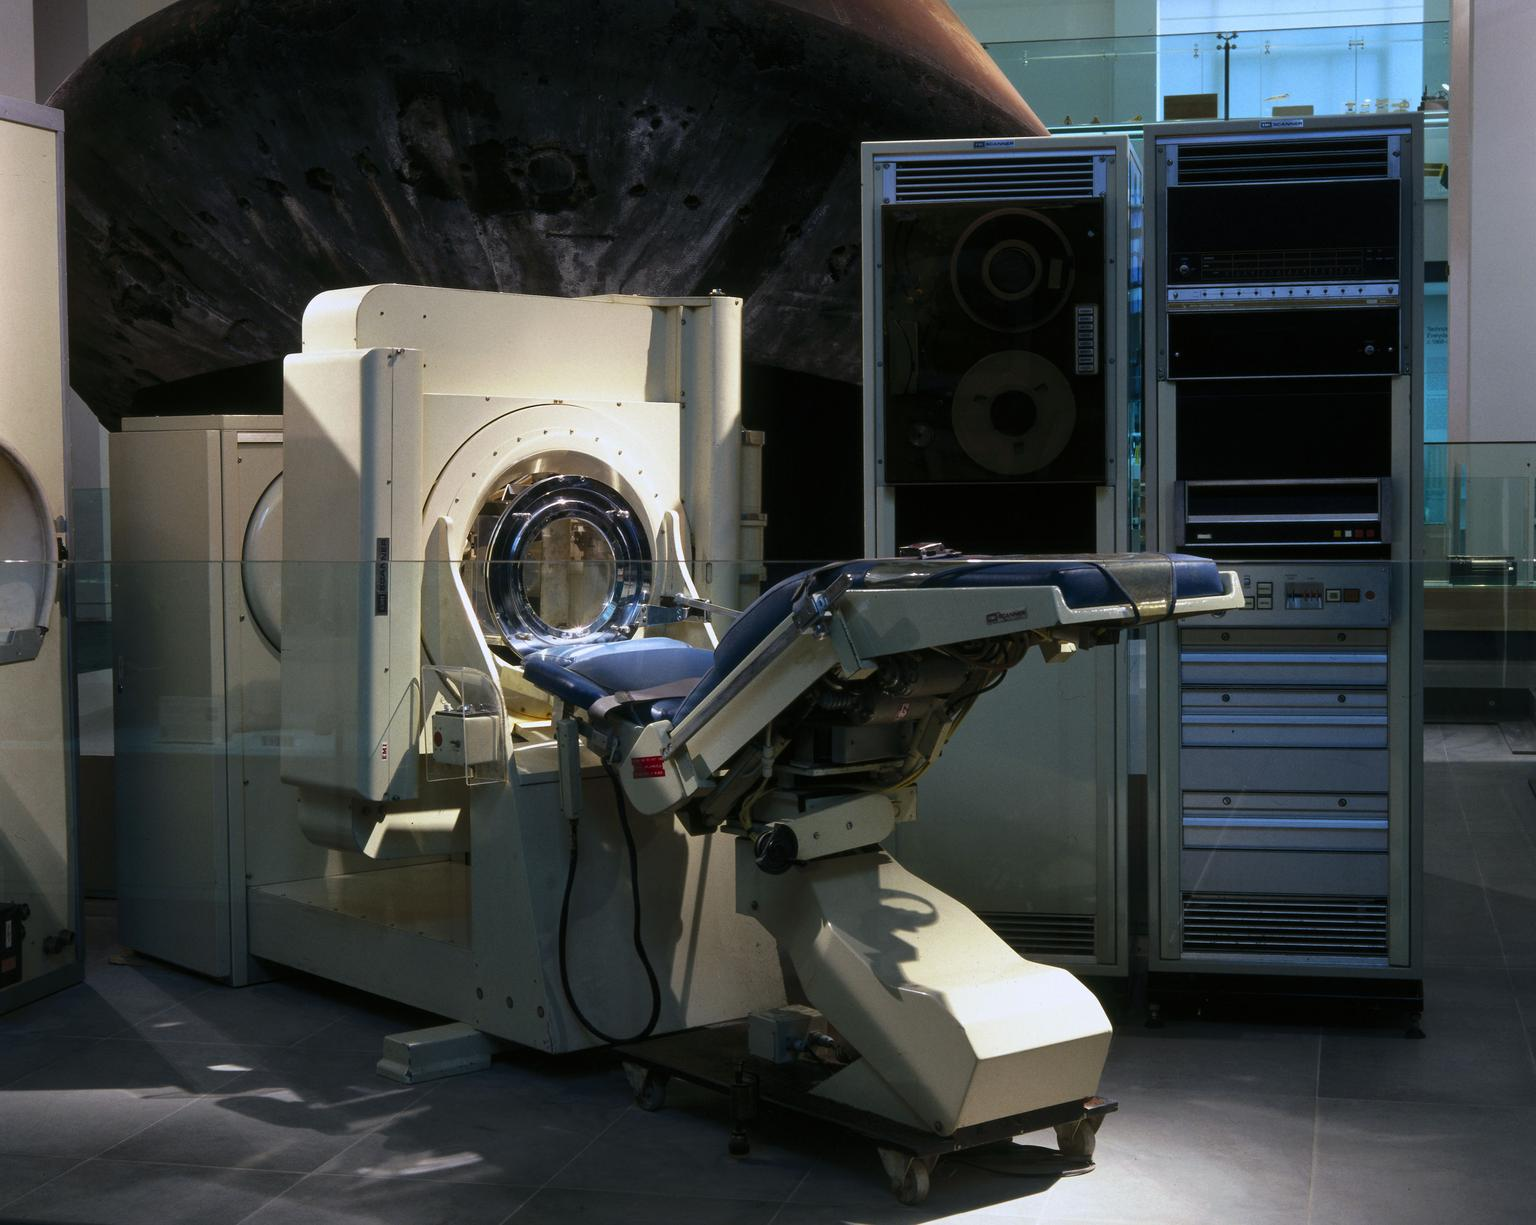
\includegraphics[width=0.2\textwidth]{images/CT.jpg}
\caption{First EMI Scanner \cite{emict}}\label{fig:CT1010}
\end{figure}

\vfill{\null}

\section{Theory} \label{sec:theory}
\subsection{X-Ray Attenuation}
In X-ray tomography, images are modelled as attenuation coefficient distributions which is a measure of how much X-ray beams are attenuated when they propagate through an object. This problem can be modeled as in Eqn. \ref{eq:radon3d} for an arbitrary object.
\begin{equation} 
	I_{measured} = I_0 e^{-\iiint\limits_{object}\mu(x,y,z)dxdydz}
	\label{eq:radon3d}
\end{equation}
When the object to be imaged is two dimensional or can be reduced to a two dimensional slice, Eqn \ref{eq:radon3d} reduces to Eqn \ref{eq:radon2d}:
\begin{equation}
	I_{measured} = I_0 e^{-\iint\limits_{slice}\mu(x,y)dxdy}
	\label{eq:radon2d}
\end{equation}
\subsection{Radon Transform}
Radon Transform computes the line integrals along the objects to obtain projections along an arbitrary angle $\theta$ for an arbitrary beam t, using the formula given in Eqn. \ref{eq:radongeneral}.
\begin{equation}
	p_{\theta}(t) = \iint\limits_{-\infty}^{\ \ \ \infty}\mu(x,y)\delta(xcos(\theta)+ysin(\theta)-t)dxdy
	\label{eq:radongeneral}
\end{equation}
This equation models the X-ray beams as parallel lines through the object. In a more practical scenario, the X-ray source is modelled as a point source and beams are projected from source to the object in fan beam shape, due to the equiangular spaced discrete detector locations. This modelling can be achieved by introducing geometric transformation between projection variables. 

\begin{figure}[h]
\centering
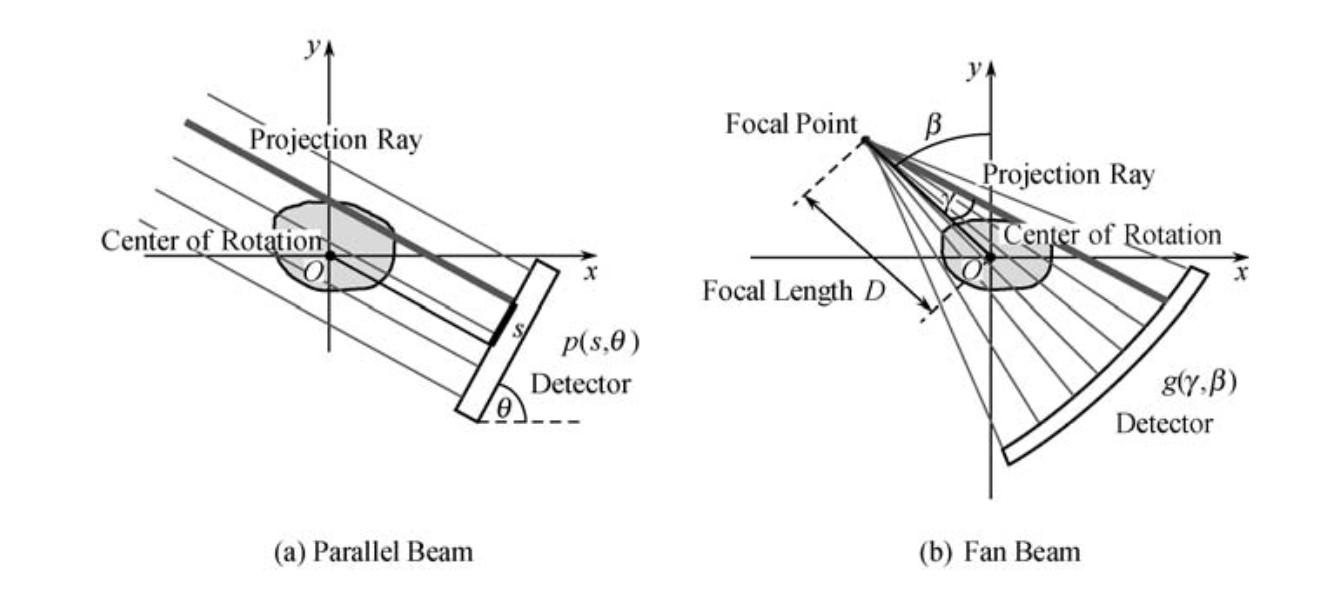
\includegraphics[width=0.4\textwidth]{images/PvsB.jpg}
\caption{Parallel Beams and Fan Beams \cite{zeng2017image}}\label{fig:PvsB}
\end{figure}

In Figure \ref{fig:PvsB}b, the projection angle with respect to center of rotation is defined as $\beta$ and the deviation from the center beam that is parallel to the $\beta$ beam is defined as $\gamma$ angles. In addition, the source to origin distance is labelled as $D$, resulting in source to detector distance of $2D$. 

With source to detector distance redefined as D and the remaining quantities defined as above, one could transform the equation in \ref{eq:radongeneral} to \ref{eq:transformedgeneral} using Eqn. \ref{eq:trans1} and \ref{eq:trans2}.
\begin{align}
	t &= D \cdot sin(\gamma) \label{eq:trans1} \\
	\theta &= \beta + \gamma \label{eq:trans2} \\
	p_{\beta}(\gamma) &= \iint\limits_{-\infty}^{\ \ \ \infty}\mu(x,y)\delta(xcos(\theta)+ysin(\theta) \label{eq:transformedgeneral} \\&-Dsin(\gamma))d\gamma d\beta \nonumber 
\end{align}

\subsection{Fourier Slice Theorem}

The Fourier slice theorem states that Fourier transform of a projection vector $S_{\theta}(\omega) = \mathcal{F}(p_{\theta}(t))$ is the section of the original image distribution's Fourier transform $\mathcal{F}(\omega,\theta)$ along the slice of angle $\theta$, which is formally described by Eqn. \ref{eq:Fslice} \cite{kak2001principles}.

\begin{equation}
	S_{\theta}(w) = \cal{F}(\omega\cos\theta,\omega\sin\theta)
	\label{eq:Fslice}
\end{equation}

\subsection{Back Projection}

According to Fourier Slice theorem, as it is formulated in \cite{kak2001principles}, the original image distribution from projections can be obtained as follows:

\begin{equation}
	f(x,y) = \int\limits_0^\pi\left[\int\limits_{-\infty}^{+\infty}S_{\theta}(\omega)|w|e^{-j2\pi{\omega}t}d\omega\right]d\theta
	\label{eq:perfectreconstruction}
\end{equation}

The term $|w|$ originates from the Jacobian of the coordinate transformation between Cartesian Space and Polar frequency variables. 

\begin{align}
	f(x,y) &= \int\limits_{-\infty}^{+\infty}\int\limits_{-\infty}^{+\infty}\mathcal{F}(u,v)e^{-j2\pi{(ux+vy)}}du{dv} \label{eq:2DFFT} \\
	u &= \omega\cos\theta \\
	v &= \omega\sin\theta \\
	du dv &= \omega d\omega d\theta \label{eq:Jacobian}
\end{align}

The factor $\omega$ in Eqn. \ref{eq:Jacobian} derives from the Jacobian as follows:
\begin{gather}
	\begin{align}
	J &= \begin{vmatrix}
		\frac{\partial u}{\partial \omega} & \frac{\partial v}{\partial \omega} \\ 
		\frac{\partial u}{\partial \theta} & \frac{\partial v}{\partial \theta} 
	\end{vmatrix} = \begin{vmatrix}
		\cos\theta & \sin\theta \\ 
		-\omega\sin\theta & \omega\cos\theta \\
	\end{vmatrix} \\
	&= \omega(\sin^2\theta + \cos^2\theta) = \omega
	\end{align}
\end{gather}

\subsection{Convolution Back Projection}
Eqn. \ref{eq:perfectreconstruction} tells us that the 1D Fourier transforms of the projection vectors should be weighted, \textit{i.e.} filtered, with $|w|$ to obtain the perfect reconstruction of the original unknown distribution. From Eqn. \ref{eq:perfectreconstruction}, one can deduce that the impulse response of the projection system is $\frac{1}{|\omega|}$, \textit{i.e.}, the components representing the high frequencies in the image distribution is attenuated when they are projected and represented in the Fourier space. 
\vfill{\null}
To overcome this low-pass effect, the projections should be filtered with the sequence having the frequency distribution $|w|$. The filter having the band-limited characteristics of above-mentioned frequency response is called Ram-Lak filter.

\begin{figure}[h]
	\centering
	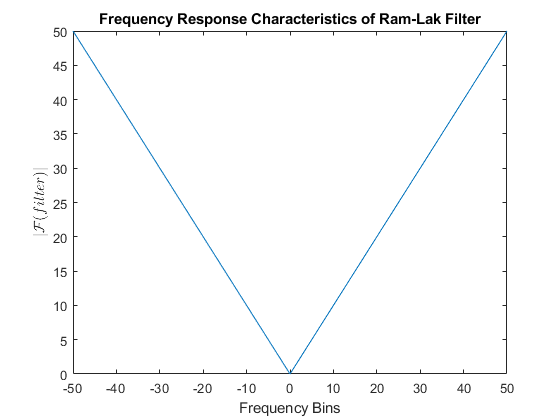
\includegraphics[width=.8\columnwidth]{images/ramlak.png}
	\caption{Ram-Lak filter response}\label{fig:barthannresp}
	\end{figure}

The sharp decrease in the Ram-Lak filter response causes ringing effect in the reconstructed images. To overcome this, the filter can be smoothed out in the higher frequency region with low-pass windows given in Figure \ref{fig:smoothingfilters}

\begin{figure}[h]
	\centering
	\begin{subfigure}[b]{0.45\columnwidth}
		\centering
	  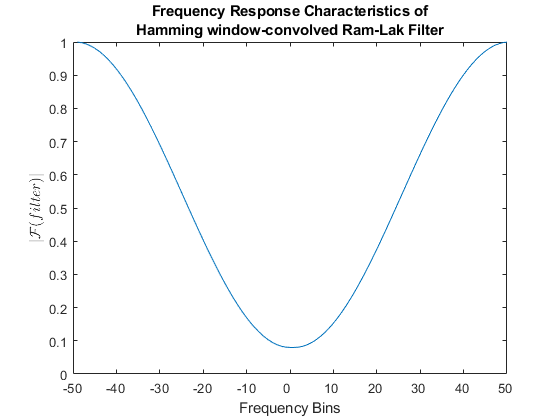
\includegraphics[width=\linewidth]{images/hamm.png}
	  \caption{Hamming window}
	  \label{fig:hamm}
	\end{subfigure}
	\begin{subfigure}[b]{0.45\columnwidth}
		\centering
	  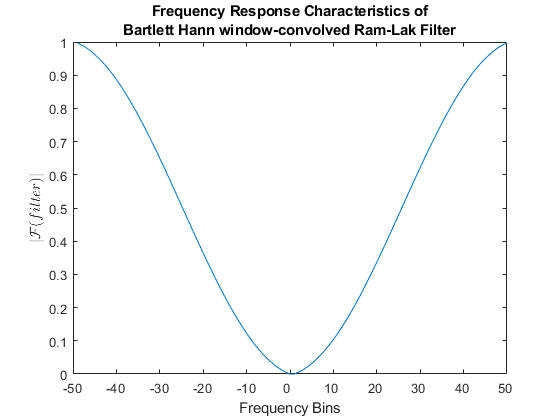
\includegraphics[width=\linewidth]{images/barthannresp.png}
	  \caption{Bart-Hann window}
	  \label{fig:bart}
	\end{subfigure}
	\caption{Smoothing window functions}
	\label{fig:smoothingfilters}
\end{figure}

Then, the resultant filter responses are as follows:

\begin{figure}[h]
	\centering
	\begin{subfigure}[b]{0.45\columnwidth}
		\centering
	  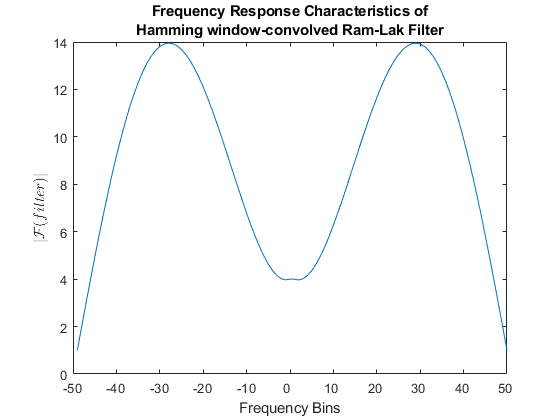
\includegraphics[width=\linewidth]{images/smoothedhamm.png}
	  \caption{Hamming \newline smoothed Ram-Lak}
	  \label{fig:smoothhamm}
	\end{subfigure}
	\begin{subfigure}[b]{0.45\columnwidth}
		\centering
	  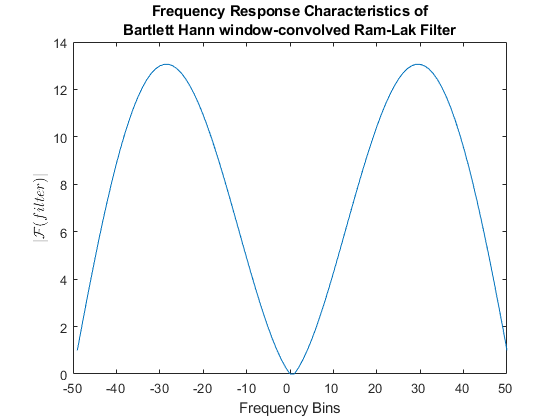
\includegraphics[width=\linewidth]{images/smoothedhann.png}
	  \caption{Bart-Hann \newline smoothed Ram-Lak}
	  \label{fig:smoothbarthann}
	\end{subfigure}
	\caption{Ram-Lak filter response smoothed out with window functions}
	\label{fig:smoothedfilters}
\end{figure}

The columns of the projection matrix of size $[\#Rays \times \#Projection Angles]$ is convolved with the filters having the responses shown in Figure \ref{fig:smoothedfilters}. This operation is called Convolution Back Projection.

\section{Implementation} \label{sec:implementation}

In this section, the computer implementation of the scientific background explained in Section \nameref{sec:theory} is going to be described.

\begin{algorithm}[h]
	\caption{Projection algorithm}
	\begin{algorithmic}
	\Procedure{Projection}{$I,N_D, L_D, L_{SD}$} 
	\State Projections = ZEROS
	\State Form the image Grid $[X(:),Y(:)]$
	   \For{Projection angle $\beta$}
	   	  \For{Fan beam angle $\gamma$}\\
			\Comment{$Line = F(x,y,\beta,\gamma)$}
			\State Calculate x intersection
			\State Calculate y intersection
			\State Sort \Comment{Regular grid}
			\State Find distance between intersections\Comment{weights}
			\State Find the corresponding pixels
			\State Calculate projection \Comment{$weights \cdot I(pixels)$}
			\State Store in projection matrix
		  \EndFor
	   \EndFor
	   \State \textbf{return Projection matrix}
	\EndProcedure
	\end{algorithmic}
	\label{alg:projection}
\end{algorithm}

The matrix returned by the procedure defined in Algorithm \ref{alg:projection} is used in Algorithm \ref{alg:backprojection} to reconstruct the image. 

\begin{algorithm}[h]
	\caption{Backprojection algorithm}
	\begin{algorithmic}
	\Procedure{Projection}{$I,N_D, L_D, L_{SD}$} 
	\State Projections = ZEROS
	\State Form the image Grid $[X(:),Y(:)]$
	   \For{Projection angle $\beta$}
	   	  \For{Fan beam angle $\gamma$}\\
			\Comment{$Line = F(x,y,\beta,\gamma)$}
			\State Calculate x intersection
			\State Calculate y intersection
			\State Sort \Comment{Regular grid}
			\State Find distance between intersections\Comment{weights}
			\State Find the corresponding pixels \Comment{Mid-points}
			\State Sum projections in the pixels \Comment{$I(pixel) += projection$}
		  \EndFor
	   \EndFor
	   \State \textbf{return Reconstructed Image}
	\EndProcedure
	\end{algorithmic}
	\label{alg:backprojection}
\end{algorithm}
\newpage
\section{Results}\label{sec:results}

Using the algorithm defined in the \nameref{sec:implementation} section, all the sample phantoms are reconstructed via Projection and Convolution Back projection algorithm. \Cref{fig:lane,fig:sqcircprojected,fig:squareprojected,fig:sheppprojected} are reconstructed utilizing the following projection parameters for angles \(0^\circ, 45^\circ, 90^\circ\):
\begin{itemize}
	\item Number of detectors = 71
	\item Number of fans = 180
	\item Source to detector distance = Image size $\times \sqrt{3}$
	\item Length of the detector = Source to detector distance 
\end{itemize}
\begin{figure}[h]
\centering
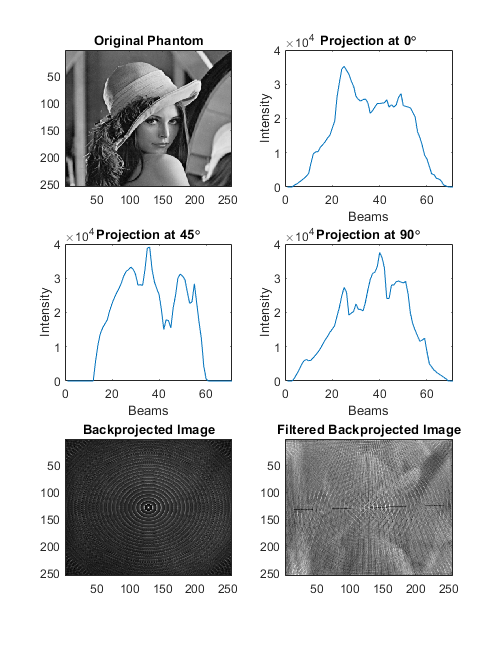
\includegraphics[width=\columnwidth,height=.3\textheight]{images/lenaprojected.png}
\caption{Projections and reconstructions of Lena phantom}\label{fig:lane}
\end{figure}
\begin{figure}[h]
	\centering
	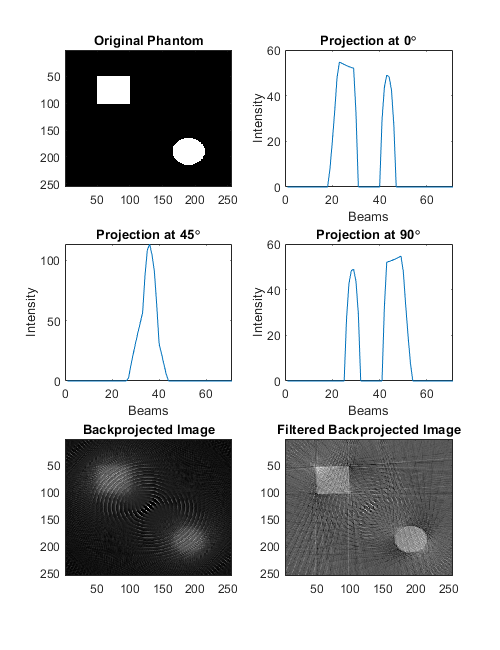
\includegraphics[width=\columnwidth,height=.3\textheight]{images/sqcircprojected.png}
	\caption{Projections and reconstructions of Square-Circle phantom}\label{fig:sqcircprojected}
\end{figure}
\begin{figure}[h]
	\centering
	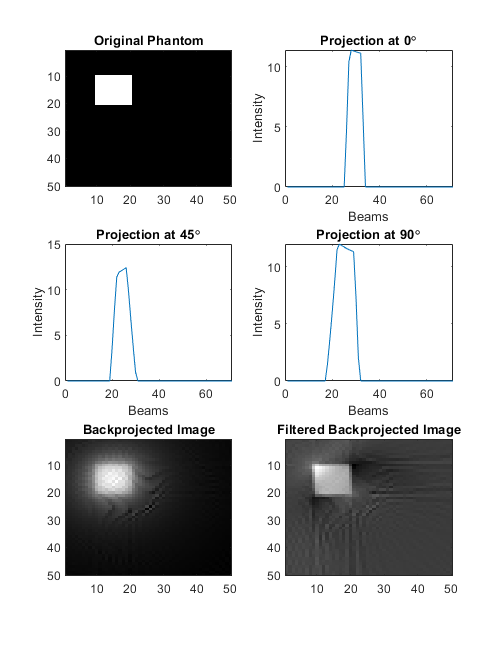
\includegraphics[width=\columnwidth,height=.3\textheight]{images/square_projected.png}
	\caption{Projections and reconstructions of Square phantom}\label{fig:squareprojected}
\end{figure}
\begin{figure}[h]
	\centering
	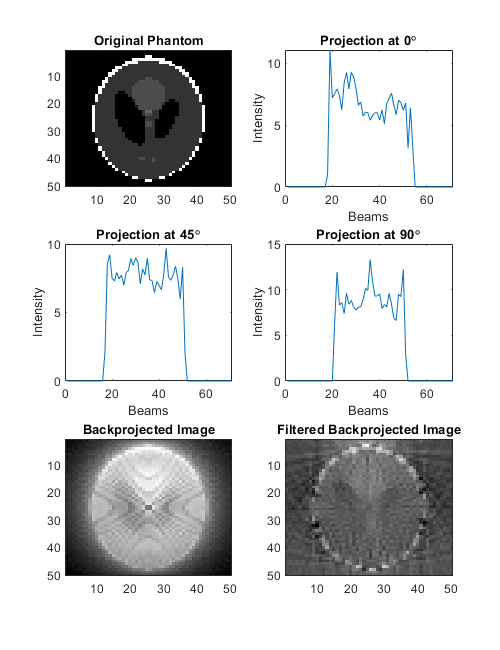
\includegraphics[width=\columnwidth,height=.3\textheight]{images/shepp_projected.png}
	\caption{Projections and reconstructions of Shepp Logan phantom}\label{fig:sheppprojected}
\end{figure}
\newpage
In addition, the effect of the parameters such as filter type, projection angle step size and number of detectors are examined using the structural similarity index \cite{wang2004image} between the gray intensity pictures of ground truth phantoms and reconstructed images. The results of these experiments are presented in \Cref{tab:filter,tab:angle,tab:beams}.
\begin{table}[h]
\centering
	\begin{tabular}{|c|c|c|c|}
		\hline 
		\diagbox{Filters}{Phantoms} & Shepp Logan & Square & Square Circle \\ 
		\hline 
		No-filter & 0.153 & 0.100 & 0.029 \\ 
		Ram-Lak & 0.231 & 0.057 & 0.032 \\ 
		BartHann & 0.246 & 0.058 & 0.044 \\ 
		Hamming & 0.244 & 0.058 & 0.043 \\ 
		\hline 
		\end{tabular}
\caption{\label{tab:filter}SSIM Index for different filter reconstructions}
\end{table}
\newpage
\begin{table}[h]
	\centering
	\begin{tabular}{|c|c|c|c|c|}
		\hline 
		\diagbox{Filters}{Phantoms} & 50 & 75 & 150 & 300 \\ 
		\hline 
		No-filter & 0.015 & 0.018 & 0.017 & 0.035 \\ 
		Ram-Lak & 0.019 & 0.019 & 0.024 & 0.039 \\ 
		BartHann & 0.027 & 0.028 & 0.034 & 0.048 \\ 
		Hamming & 0.026 & 0.028 & 0.033 & 0.048 \\ 
		\hline 
		\end{tabular}
	\caption{\label{tab:beams}SSIM Index for different number of beams}
\end{table}
\begin{table}[h]
	\centering
	\begin{tabular}{|c|c|c|c|c|}
		\hline 
		\diagbox{Filters}{Phantoms} & 2 & 1 & 0.5 & 0.25 \\ 
		\hline 
		No-filter & 0.022 & 0.029 & 0.030 & 0.030 \\ 
		Ram-Lak & 0.025 & 0.032 & 0.039 & 0.043 \\ 
		BartHann & 0.028 & 0.044 & 0.049 & 0.048 \\ 
		Hamming & 0.027 & 0.043 & 0.048 & 0.048 \\ 
		\hline 
		\end{tabular}
	\caption{\label{tab:angle}SSIM Index for different angles}
\end{table}
The experiments show that the imaging parameters may affect the reconstructed imaging quality significantly with respect to the case where the parameters are not carefully selected. One example image reconstructed with $0.5^\circ$ angle step size and 200 detectors can be seen in \Cref{fig:sheppimproved,fig:sqcircimproved},
\begin{figure}[h]
	\centering
	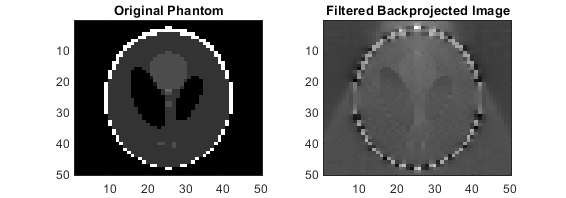
\includegraphics[width=\columnwidth,height=.15\textheight]{images/shepp_improved.png}
	\caption{Improved reconstruction of Shepp Logan phantom}\label{fig:sheppimproved}
\end{figure}
\begin{figure}[h]
	\centering
	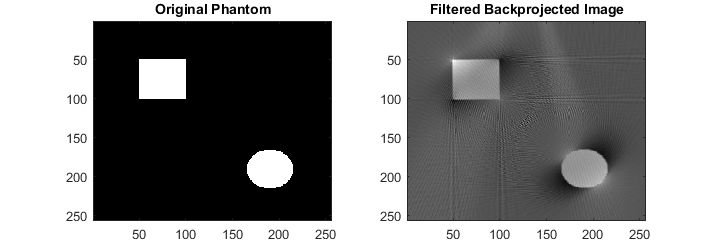
\includegraphics[width=\columnwidth,height=.15\textheight]{images/sqcircimproved.png}
	\caption{Improved reconstruction of Square Circle phantom}\label{fig:sqcircimproved}
\end{figure}




\section{Discussion} \label{sec:discuss}
Some discussion here



\printbibliography
\end{document}
